\section{Combining Transcription and Prediction}
\label{sec:combination}

%\textit{NOTE: Could describe how the predictions made by the MLM influence the transcription of the  AMT system in this section.}

In this section, we describe the process for combining the acoustic model with the music language model for deriving an improved transcription. Firstly, the input music signal is transcribed using the process described in Section \ref{sec:transcription}. The resulting piano-roll representation of the transcription system is considered to be a sequence $p_1, p_2, \ldots, p_T$ that is placed as input to the MLM presented in Section \ref{sec:prediction}. For the RNN-NADE, we compute the probability $P(p_i|\mathbf{v_{<i}})$ for all time frames, and use that as prior information for the combined model, with the prior information  denoted as $P_{\mathit{MLM}}(p,t)$, where $P_{\mathit{MLM}}(p=i,t)=P(p_i|\mathbf{p_{<i}})$. For the RNN, the prediction output is directly denoted as $P_{\mathit{MLM}}(p,t)$, since pitch probabilities are independent.

As shown in \cite{Smaragdis2009}, PLCA-based models use multinomial distributions; since the Dirichlet distribution is conjugate to the multinomial, a Dirichlet prior can be used to enforce structure on the pitch activation distribution $P_{t}(p)$. Following the procedure of \cite{Smaragdis2009}, we define the Dirichlet hyperparameter for the pitch activation as:
\begin{equation}
 \alpha_{t}(p) = \frac{P(p|t)P_{\mathit{MLM}}(p,t)}{\sum_{p}P(p|t)P_{\mathit{MLM}}(p,t)}
\end{equation}
where $\alpha(p|t)$ essentially is a pitch activation probability which is filtered through a pitch indicator function computed from the symbolic prediction step (the denominator is simply for normalisation purposes).

The recording is then re-transcribed, using as aditional information the prior computed from the transcription step. The modified update for the pitch activation which replaces (\ref{eq:MStepTranscription}) is given by:
\begin{equation}
 P_{t}(p) = \frac{\sum_{\omega,f,s}P_{t}(p,f,s|\omega)V_{\omega,t}+\kappa\alpha(p|t)}{\sum_{p,\omega,f,s}P_{t}(p,f,s|\omega)V_{\omega,t}+\kappa\alpha(p|t)} \label{eq:modifiedMStepPitchActivation}
\end{equation}
where $\kappa$ is a weight parameter expressing how much the prior should be imposed; as in \cite{Smaragdis2009}, the weight decreases from 1 to 0 throughout the iterations. In a larger context, the transcription creates a symbolic prediction, which in turn improves the subsequent re-transcription of the music signal. An overview of the complete transcription-prediction system architecture can be seen in Fig. \ref{fig:system}.

\begin{figure*}
\begin{center}
\resizebox{340pt}{!}{
 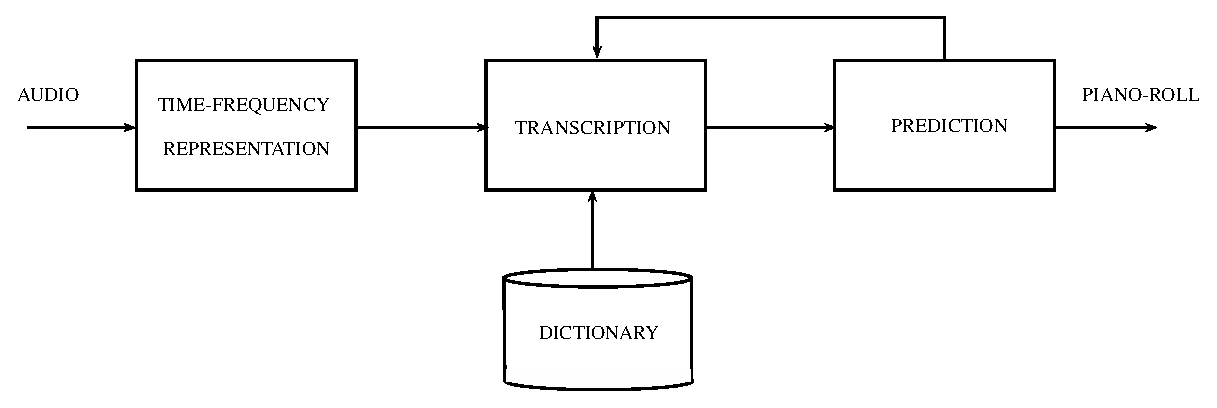
\includegraphics{figures/FigSystem.eps} 
 }
 \caption{Proposed system diagram.}
 \end{center}
 \label{fig:system}
\end{figure*}
